% Use the standalone as the document class with an option which allows specifying the border.
\documentclass[border = 10pt]{standalone}

% Allow to entering comfortably English.
\usepackage[T1]{fontenc}
\usepackage[utf8]{inputenc}
\usepackage[french]{babel}

% 
\usepackage{xcolor}
\definecolor{color0}{HTML}{372639}
\definecolor{color1}{HTML}{C2A4C0}
\definecolor{color2}{HTML}{816288}
\definecolor{color3}{HTML}{C6926C}
\definecolor{color4}{HTML}{D5BEA9}
\definecolor{color5}{HTML}{DBCAD3}


%
\usepackage{tikz}
%
\usetikzlibrary{mindmap}
%
\usetikzlibrary{shadows}

\usepackage[hidelinks, pdfencoding = auto]{hyperref}

\usetikzlibrary{backgrounds}

\usepackage{wallpaper}

\begin{document}
	
%\ThisCenterWallPaper{}{./figures/Social_Network_Analysis_Visualization_transparent.png}

\centering

\begin{tikzpicture}

\begin{scope}
	[
		mindmap,
		every node/.style =
		{
			concept,
			execute at begin node = \hskip 0pt
		},
		root concept/.append style =
		{
			concept color = color0,
			rectangle,
			rounded corners = 2em,
			fill = color5!10,
			line width = 0.5em,
			text width = 40em,
			text = color0,
			font = \huge\scshape,
			inner sep = 2em
		}
	]
	\node [root concept] (Nom de projet)
	at (0em, 0em) {{SYSTÈMES INTELLIGENTS \\POUR LA TRANSMISSION DES \\HUMANITÉS NUMÉRIQUES ET \\POUR LA RECHERCHE EN SANTÉ}};
\end{scope}

\begin{scope}
	[
		mindmap,
		text = color0,
		grow cyclic,
		every node/.style =
			{
				concept,
				concept color = color1!50,
				text = color0,
				execute at begin node = \hskip 0pt
			},
		root concept/.append style =
			{
				concept color = color1,
				draw = color1!75,
				fill = color1!10,
				line width = 1em,
				text width = 20em,
				text = color0,
				font = \LARGE\scshape,
				inner sep = 0pt
			},
		level 1/.append style =
			{
				concept color = color1,
				draw = color1!50,
				fill = color1!5,
				line width = 0.5em,
				text width = 18em,
				text = color0,
				font = \Large\bfseries,
				inner sep = 0pt
			},
		level 2/.append style =
			{
				concept color = color1,
				draw = color1!50,
				fill = color1!5,
				line width = 0.5em,
				text width = 16em,
				text = color0,
				font = \large\bfseries,
				inner sep = 0pt
			}
	]

	\node [root concept, text width = 20em] (UBFC)
		at (-60em, 35em)
			{
\includegraphics[width = 0.95\textwidth]{./logos/logo UBFC.png}}
		child [grow = 90, level distance = 30em, concept color = color1!50]
			{
				node [level 1, text width = 18em] (UFC) {
\includegraphics[width = 0.9\textwidth]{./logos/logo UFC.png}}
			}
		child [grow = -90, level distance = 30em, concept color = color1!50]
			{
				node [level 1, text width = 18em, inner sep = -0.5em] (I-SITE BFC) {
\includegraphics[width = 0.65\textwidth]{./logos/logo I-SITE BFC.png}}
			}
		child [grow = 0, level distance = 30em, concept color = color1!50]
			{
				node [level 1, text width = 18em, inner sep = -1em] (LLC) {\LARGE{Pôle Lettres, \\Langues et \\Communication} \\\vspace{1em} \Huge{- LLC}}
				child [grow = 90, level distance = 30em, concept color = color1!50]
				{
					node [level 2, text width = 18em] (LECLA) {
\includegraphics[width = 0.95\textwidth]{./logos/logo LECLA.png}}
				}
				child [grow = 45, level distance = 30em, concept color = color1!50]
				{
					node [level 2, text width = 18em, inner sep = -1em] (MSH) {
\includegraphics[width = 0.85\textwidth]{./logos/logo MSH.png}}
				}
				child [grow = 0, level distance = 30em, concept color = color1!50]
				{
					node [level 2, text width = 18em, inner sep = -0.75em] (ELLIADD) {
\includegraphics[width = 0.8\textwidth]{./logos/logo ELLIADD.png}}
					child [grow = 0, level distance = 30em, concept color = color1!50]
					{
						node [level 2, text width = 18em, inner sep = -1.5em] (HULIN) {
\includegraphics[width = \textwidth]{./profile/HULIN.png}}
					}
				}
			};
	\node[annotation, left,  concept color = color1, draw = color1!50, fill = color1!5, line width = 0.25em, text width = 20em, text = color0, font = \Large\bfseries, inner sep = 1em]
		at (-25em, 2em)
			{Ce projet s'inscrit naturellement dans l'axe 1 de l'I-SITE consacré aux systèmes intelligents, ainsi que dans l'axe 3 sur la santé grâce à l'approche comparative des usages.};
	\node[annotation, concept color = color1, draw = color1!50, fill = color1!5, line width = 0.25em, text width = 42em, text = color0, font = \Large\bfseries, inner sep = 1em] 
		at (-30em, 18.5em)
		{Ce projet concerne tous les pôles de UBFC : la valorisation des corpus dans le champ de l'enseignement des HN mobilisera les pôles AL, DTMS et LLC ; l'expérience en HN et en web sémantique mobilise le pôle CCM et sur son axe transversal SEISM portant sur la recherche en éducation ; le design de la plateforme et son évaluation, le pôle ERCOS.};
	\node[annotation, concept color = color1, draw = color1!50, fill = color1!5, line width = 0.25em, text width = 30em, text = color0, font = \Large\bfseries, inner sep = 1em]
		at(-20em, 79em)
			{Cette offre de thèse proposée par le laboratoire ELLIADD et l'école doctorale LECLA.};
	\node[annotation, concept color = color1, draw = color1!50, fill = color1!5, line width = 0.25em, text width = 30em, text = color0, font = \Large\bfseries, inner sep = 1em]
		at(-4em, 71em)
			{Ce projet s'inscrit dans le paradigme de la transmission des pôles thématiques de la fédération des MSH BFC.};
	\node[annotation, concept color = color1, draw = color1!50, fill = color1!5, line width = 0.25em, text width = 8em, text = color0, font = \Large\bfseries, inner sep = 1em]
		at(0em, 18em)
			{Ce projet rattaché au laboratoire ELLIADD.};
	\begin{pgfonlayer}{background}
		\draw [densely dashed] 
			(Nom de projet)
				edge [color = color1!50, line width = 1em] (I-SITE BFC)
				edge [color = color1!50, line width = 1em] (MSH)
				edge [color = color1!50, line width = 1em] (ELLIADD)
				edge [color = color1!50, line width = 1em] (UBFC)
				edge [color = color1!50, line width = 1em] (LECLA);
	\end{pgfonlayer}
\end{scope}

\begin{scope}
	[
		mindmap,
		text = color0,
		grow cyclic,
		every node/.style =
		{
			concept,
			concept color = color2!50,
			text = color0,
			execute at begin node = \hskip 0pt
		},
		root concept/.append style =
		{
			concept color = color2,
			draw = color2!75,
			fill = color2!10,
			line width = 1em,
			text width = 20em,
			text = color0,
			font = \LARGE\scshape,
			inner sep = 0pt
		},
		level 1/.append style =
		{
			concept color = color2,
			draw = color2!50,
			fill = color2!5,
			line width = 0.5em,
			text width = 18em,
			text = color0,
			font = \Large\bfseries,
			inner sep = 0pt
		},
		level 2/.append style =
		{
			concept color = color2,
			draw = color2!50,
			fill = color2!5,
			line width = 0.5em,
			text width = 16em,
			text = color0,
			font = \large\bfseries,
			inner sep = 0pt
		}
	]

	\node [root concept, text width = 20em, inner sep = -0.5em] (HUMANE)
		at (50em, 50em)
			{\Huge{Projet \\HUMANE} \\\vspace{0.5em}\Large{\og Humanités Numériques \\pour l'Éducation \fg}}
		child [grow = 135, level distance = 30em, concept color = color2!50]
			{
				node [level 1, text width = 18em, inner sep = -0.5em] (MENJS) {
\includegraphics[width = 0.8\textwidth]{./logos/logo MENJS.png}}
			}
		child [grow = -45, level distance = 30em, concept color = color2!50]
			{
				node [level 1, text width = 18em] (GIS 2IF) {
\includegraphics[width = 0.9\textwidth]{./logos/logo GIS 2IF.png}}
			}
		child [grow = 0, level distance = 30em, concept color = color2!50]
			{
				node [level 1, text width = 18em] (canope) {
\includegraphics[width = 0.9\textwidth]{./logos/logo canope.png}}
			}
		child [grow = 45, level distance = 30em, concept color = color2!50]
			{
				node [level 1, text width = 18em, inner sep = -2em] (humanistica) {
\includegraphics[width = 0.9\textwidth]{./logos/logo humanistica.png}}
			};
	\node[annotation, concept color = color2, draw = color2!50, fill = color2!5, line width = 0.25em, text width = 15em, text = color0, font = \Large\bfseries, inner sep = 1em]
		at(48em, 72em)
			{Le projet HUMANE est financé par la Direction Numérique pour l'Éducation du Ministère de l'Éducation Nationale.};
	\node[annotation, left,  concept color = color2, draw = color2!50, fill = color2!5, line width = 0.25em, text width = 12em, text = color0, font = \Large\bfseries, inner sep = 1em]
		at (22em, 22em)
			{7 chercheurs de ELLIADD travaillent déjà au projet HUMANE.};
	\node[annotation, left,  concept color = color2, draw = color2!50, fill = color2!5, line width = 0.25em, text width = 22em, text = color0, font = \Large\bfseries, inner sep = 1em]
		at (27em, 52em)
			{\LARGE\bfseries{M. Thibaud HULIN} \\\Large\bfseries{Directeur de thèse, qui dirigera cette thèse en tant que membre d'ELLIADD et le co-animateur académique pour la Franche-Comté.}};
	\begin{pgfonlayer}{background}
		\draw [densely dashed] 
			(HUMANE)
				edge [color = color2!50, line width = 1em] (Nom de projet)
				edge [color = color2!50, line width = 1em] (ELLIADD)
				edge [color = color2!50, line width = 1em] (HULIN);
	\end{pgfonlayer}
\end{scope}


\begin{scope}
	[
		mindmap,
		text = color0,
		grow cyclic,
		every node/.style =
		{
			concept,
			concept color = color3!50,
			text = color0,
			execute at begin node = \hskip 0pt
		},
		root concept/.append style =
		{
			concept color = color3,
			draw = color3!75,
			fill = color3!10,
			line width = 1em,
			text width = 20em,
			text = color0,
			font = \LARGE\scshape,
			inner sep = 0pt
		},
		level 1/.append style =
		{
			concept color = color3,
			draw = color3!50,
			fill = color3!5,
			line width = 0.5em,
			text width = 18em,
			text = color0,
			font = \Large\bfseries,
			inner sep = 0pt
		},
		level 2/.append style =
		{
			concept color = color3,
			draw = color3!50,
			fill = color3!5,
			line width = 0.5em,
			text width = 16em,
			text = color0,
			font = \large\bfseries,
			inner sep = 0pt
		}
	]
	
	\node [root concept, text width = 20em] (Co-tutelle Internationale)
		at (12em, -40em)
			{\Huge{Co-tutelle} \\\huge{Internationale}}
		child [grow = 45, level distance = 30em, concept color = color3!50]
			{
				node [level 1, text width = 18em] (Laval University) {
\includegraphics[width = 0.95\textwidth]{./logos/logo Laval University.png}}
				child [grow = 90, level distance = 30em, concept color = color3!50]
				{
					node [level 2, text width = 18em, inner sep = 0.25em] (LAVAL FSE) {
\includegraphics[width = 0.95\textwidth]{./logos/loge LAVAL FSE.png}}
				}
			}
		child [grow = 180, level distance = 30em, concept color = color3!50]
			{
				node [level 1, text width = 18em, inner sep = -2em] (RPI) {
\includegraphics[width = 0.95\textwidth]{./logos/logo RPI.png}}
				child [grow = 180, level distance = 30em, concept color = color3!50]
				{
					node [level 2, text width = 18em, inner sep = -1.5em] (McGuinness) {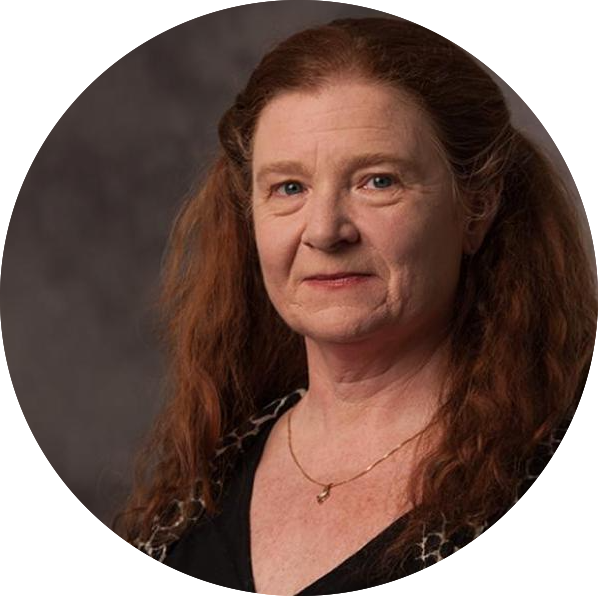
\includegraphics[width = \textwidth]{./profile/McGuinness.png}}
				}
				child [grow = 135, level distance = 30em, concept color = color3!50]
				{
					node [level 2, text width = 18em, inner sep = -1.5em] (McCusker) {
\includegraphics[width = \textwidth]{./profile/McCusker.png}}
				}
			};%Co-directrice Deborah Louise McGuinness
	\node[annotation, left,  concept color = color3, draw = color3!50, fill = color3!5, line width = 0.25em, text width = 45em, text = color0, font = \Large\bfseries, inner sep = 1em]
		at (20em, -15em)
			{\LARGE\bfseries{M. Jamie McCusker, la co-tutelle de projet} \\\Large\bfseries{Le directeur de Data Operation à l'IPR et le principal développeur du projet Whyis. \\À noter que Whyis est développé dans le cadre de l'Institute for Data Exploration and Applications (RPI-IDEA), bien sûr utilisé dans le cadre de la recherche sur le COVID-19.}};
	\node[annotation, left,  concept color = color3, draw = color3!50, fill = color3!5, line width = 0.25em, text width = 16em, text = color0, font = \Large\bfseries, inner sep = 1em]
		at (-50em, -22em)
			{\LARGE\bfseries{Mme Deborah L. McGuinness} \\\Large\bfseries{La co-directrice, contributrice du W3C, leader dans le web sémantique et en sciences cognitives.}};
\end{scope}

\begin{scope}
	[
		mindmap,
		text = color0,
		grow cyclic,
		every node/.style =
		{
			concept,
			concept color = color4!50,
			text = color0,
			execute at begin node = \hskip 0pt
		},
		root concept/.append style =
		{
			concept color = color4,
			draw = color4!75,
			fill = color4!10,
			line width = 1em,
			text width = 20em,
			text = color0,
			font = \LARGE\scshape,
			inner sep = 0pt
		},
		level 1/.append style =
		{
			concept color = color4,
			draw = color4!50,
			fill = color4!95,
			line width = 0.5em,
			text width = 16em,
			text = color4!5,
			font = \Large\bfseries,
			inner sep = 0pt
		},
		level 2/.append style =
		{
			concept color = color4,
			draw = color4!50,
			fill = color4!5,
			line width = 0.5em,
			text width = 16em,
			text = color0,
			font = \large\bfseries,
			inner sep = 0pt
		}
	]

	\node [level 1, text width = 18em, inner sep = -2em] (E3)
		at (80em, -15em)
			{\LARGE{Étape 3 \\design de la \\plateforme}}
		child [grow = 135, level distance = 20em, concept color = color4!50]
			{
				node [level 1, text width = 18em, inner sep = -2em] (E2) {\LARGE{Étape 2 \\construction \\des données}}
				child [grow = 45, level distance = 20em, concept color = color4!50]
				{
					node [level 1, text width = 18em, inner sep = -2em] (E1) {\LARGE{Étape 1 \\état de l'art}}
				}
			}
		child [grow = -135, level distance = 20em, concept color = color4!50]
			{
				node [level 1, text width = 18em, inner sep = -2.5em] (E4) {\LARGE{Étape 4 \\implantation \\de l'ontologie}}
				child [grow = -45, level distance = 20em, concept color = color4!50]
				{
					node [level 1, text width = 18em, inner sep = -2em] (E5) {\LARGE{Étape 5 \\test \\\& \\évaluation}}
				}
			};
	\node[annotation, left,  concept color = color4, draw = color4!50, fill = color4!5, line width = 0.25em, text width = 12em, text = color0, font = \Large\bfseries, inner sep = 1em]
		at (60em, 20em)
			{Cette étape consistera à construire l'ontologie via des séances de focus groups avec les praticiens et chercheurs du projet HUMANE, et avec l'équipe de l'université de Laval (Canada).};
	\node[annotation, left,  concept color = color4, draw = color4!50, fill = color4!5, line width = 0.25em, text width = 20em, text = color0, font = \Large\bfseries, inner sep = 1em]
		at (70em, -15em)
			{Le transfert d'expérience sera fait via l'équipe américaine à l'IPR en co-tutelle de thèse.};
	\node[annotation, left,  concept color = color4, draw = color4!50, fill = color4!5, line width = 0.25em, text width = 20em, text = color0, font = \Large\bfseries, inner sep = 1em]
		at (55em, -35em)
			{Étape collaborative, vise à implanter l'ontologie et à développer les services de la plateforme.};
	\begin{pgfonlayer}{background}
		\draw [densely dashed] 
			(E2)
			edge [color = color4!50, line width = 1em] (HUMANE)
			edge [color = color4!50, line width = 1em] (LAVAL FSE)
			(E3)
			edge [color = color4!50, line width = 1em] (RPI)
			(E4)
			edge [color = color4!50, line width = 1em] (RPI)
			;
	\end{pgfonlayer}
\end{scope}

\end{tikzpicture}

\end{document}
